\subsection{Internal skein algebras}\label{SectASigma}
When a surface has a boundary edge, one can push a little disk inside the surface from this boundary edge. This process induces an action of the skein category of the disk on the skein category of the surface. Namely, ${\rm Sk}_\mathcal{V}(\Sigma)$ is a ${\rm Sk}_\mathcal{V}\big(\mathbb{R}^2\big)$-module category, see \cite[Sections~3.2]{Cooke}. In this situation there is a notion of internal $\Hom$ objects that encode entirely in ${\rm Sk}_\mathcal{V}\big(\mathbb{R}^2\big)$ the behavior of objects of ${\rm Sk}_\mathcal{V}\big(\mathbb{R}^2\big)$ seen in ${\rm Sk}_\mathcal{V}(\Sigma)$ by the action. Namely for fixed $V,W \in {\rm Sk}_\mathcal{V}(\Sigma)$ one has $\Hom_{{\rm Sk}_\mathcal{V}(\Sigma)}(X \rhd V,W) \simeq \Hom_{{\rm Sk}_\mathcal{V}(\mathbb{R}^2)}(X, \underline{\Hom}(V,W))$ naturally in $X$, see \cite[Section~7.9]{EGNO}. However, such an object does not always exist in ${\rm Sk}_\mathcal{V}\big(\mathbb{R}^2\big)$, and actually lives in its free cocompletion. The internal skein algebra $A_\Sigma$ of the surface is the internal endomorphism algebra of the empty set $\underline{\Hom}(\varnothing,\varnothing)$, see~\cite{Gunningham} or~\cite{BBJ} together with \cite{Cooke}. This means one can understand ribbon graphs in ${\rm Sk}_\mathcal{V}(\Sigma)$ with boundary points on the bottom and near the boundary edge as morphisms in (the free cocompletion of) ${\rm Sk}_\mathcal{V}\big(\mathbb{R}^2\big)$ with target $A_\Sigma$.

Note that in \cite{Cooke}, \cite{BBJ} and \cite{Gunningham} one uses a right ${\rm Sk}_\mathcal{V}\big(\mathbb{R}^2\big)$-action and we use a left ${\rm Sk}_\mathcal{V}\big(\mathbb{R}^2\big)$-action here. See Section~\ref{SectMultiEdges} for more details.

\begin{Definition}\label{algStrOnIntHom}
Let $\mathcal{A}$ be a $k$-linear monoidal category and $\mathcal{M}$ a left $\mathcal{A}$-module category. Let~$M_1$ and~$M_2$ be two objects of~$\mathcal{M}$. The internal $\Hom$ of $M_1$ and~$M_2$ with respect to the $\mathcal{A}$-module structure is an object $\undHom(M_1,M_2)\in \mathcal{A}$
equipped with a natural isomorphism $\eta\colon \Hom_\mathcal{M}(-\rhd M_1,M_2) \tilde{\to} \Hom_\mathcal{A}(-,\undHom(M_1,M_2))$. It is unique up to canonical isomorphism when it exists.
When all involved internal $\Hom$ objects exist, one can define: the eva\-lua\-tion map ${\rm ev}_{M_1,M_2}\colon \undHom(M_1,M_2) \rhd M_1\to M_2$ is the image under $\eta^{-1}$ of ${\rm Id}_{\undHom(M_1,M_2)}$ and the composition map $c\colon \undHom(M_2,M_3) \otimes \undHom(M_1,M_2) \to \undHom(M_1,M_3)$ is the image under~$\eta$ of the morphism ${\rm ev}_{M_2,M_3} \circ ({\rm Id}_{\undHom(M_2,M_3)} \rhd {\rm ev}_{M_1,M_2})\colon (\undHom(M_2,M_3) \otimes \undHom(M_1,M_2))\rhd M_1 \to \undHom(M_2,M_3) \rhd$ $M_2\to M_3$.
In~particular, an internal endomorphism $\undEnd(M) := \undHom(M,M)$ is an algebra object in~$\mathcal{A}$, with unit the morphism $1_\mathcal{A} \to \undEnd(M)$ associated with ${\rm Id}_M$.
\end{Definition}

The functor $\Hom_\mathcal{M}(-\rhd M_1, M_2)\colon\mathcal{A}^{\rm op} \to {\rm Vect}_k$ cannot always be represented in $\mathcal{A}$. However, it is always an object of its free cocompletion.
\begin{Definition}
The 2-category ${\rm Cocomp}_k$ has objects essentially small $k$-linear cocomplete categories and morphisms $k$-linear cocontinuous functors between them, i.e., functors preserving colimits and natural transformations between functors.
It is symmetric monoidal with the Kelly tensor product $\boxtimes$ for cocomplete categories, which is characterized by
\[
\Hom_{{\rm Cocomp}_k}(\mathcal{A} \boxtimes \mathcal{B},\mathcal{C}) \simeq \Hom_{{\rm Cocomp}_k}(\mathcal{A},\Hom_{{\rm Cocomp}_k}(\mathcal{B},\mathcal{C})) \simeq {\rm Cocont}(\mathcal{A},\mathcal{B};\mathcal{C}),
\]
see \cite[Section~6.5]{Kelly2} and \cite[Theorem~2.45]{Ramos}.

The free cocompletion of a $k$-linear category $\mathcal{C}$ is a cocomplete category $\Free(\mathcal{C}) \in {\rm Cocomp}_k$ together with a functor $i\colon \mathcal{C} \to \Free(\mathcal{C})$ which is initial among functors to a $k$-linear cocomplete category. Namely, $i_*\colon \Hom_{{\rm Cat}_k}(\mathcal{C},\mathcal{D}) \to \Hom_{{\rm Cocomp}_k}(\Free(\mathcal{C}),\mathcal{D})$ is an equivalence of categories for any $\mathcal{D}\in {\rm Cocomp}_k$. The free cocompletion $\Free(\mathcal{C})$ is unique up to essentially unique equivalence.
\end{Definition}

\begin{Remark}\label{rmkFreeIsPresheaves}
A standard choice for the free cocompletion is the presheaf category $[\mathcal{C}^{\rm op},{\rm Vect}_k]$, in which $\mathcal{C}$ embeds by the Yoneda embedding. Moreover for any other choice of free cocompletion~$\hat{\mathcal{C}}$, the canonical equivalence is given by
\[
R\colon\ \begin{cases}
\hat{\mathcal{C}}  \to  [\mathcal{C}^{\rm op},{\rm Vect}_k],
\\
X \mapsto  \Hom_{\hat{\mathcal{C}}}(i(-),X).\end{cases}
\]
See \cite[Section~2.2]{Dugger} for more details. From now on, we assume that we made this standard choice and set $\Free(\mathcal{C}) := [\mathcal{C}^{\rm op},{\rm Vect}_k]$.
Note that every object $C$ of $\mathcal{C}$ seen as an object of $\Free(\mathcal{C})$ is compact projective, i.e., the functor $\Hom_{\Free(\mathcal{C})}(C,-)$ is cocontinuous.
\end{Remark}

It is then easy to verify that the free cocompletion $\Free\colon {\rm Cat}_k \to {\rm Cocomp}_k$ is a symmetric monoidal functor. Hence if $\mathcal{A} \in {\rm Cat}_k$ is a monoidal $k$-linear category and $\mathcal{M}$ an $\mathcal{A}$-module category, after free cocompletions $\Free(\mathcal{A})$ is again monoidal and $\Free(\mathcal{M})$ is a $\Free(\mathcal{A})$-module category.

\begin{Proposition}\label{propIntHomFree}
Let $\mathcal{A} \in {\rm Cat}_k$ be a monoidal $k$-linear category, $\mathcal{M}$ an $\mathcal{A}$-module category and~$M_1$, $M_2$ two objects of $\mathcal{M}$. The presheaf $F= \Hom_\mathcal{M}(-\rhd M_1,M_2) \in \Free(\mathcal{A})$ is the internal $\Hom$ object of $M_1$ and $M_2$ $($seen as objects of $\Free(\mathcal{M}))$ with respect to the $\Free(\mathcal{A})$-module structure.
\end{Proposition}

\begin{proof}
For the ``small'' objects $A \in \mathcal{A} \hookrightarrow \Free(\mathcal{A})$, the isomorphism $\Hom_{\Free(\mathcal{A})}(A,F)\simeq F(A) := \Hom_{\mathcal{M}}(A\rhd M_1,M_2)$ is given by the Yoneda lemma.
Now any object $X\in\Free(\mathcal{A})$ is obtained as a~colimit of such small objects, $X = \colim_i A_i$, $A_i \in \mathcal{A}$, by the co-Yoneda lemma. Then it is straight\-forward to check that
\begin{gather*}
\Hom_{\Free(\mathcal{A})}(X,F) \simeq \lim_i \Hom_{\Free(\mathcal{A})}(A_i,F) \simeq \lim_i \Hom_{\Free(\mathcal{M})}(A_i \rhd M_1,M_2)
\\ \hphantom{\Hom_{\Free(\mathcal{A})}(X,F)}
{}\simeq \Hom_{\Free(\mathcal{M})}(\colim_i (A_i \rhd M_1),M_2) \simeq \Hom_{\Free(\mathcal{M})}(X \rhd M_1,M_2).
\end{gather*}
Here we kept the notation $\rhd$ for its essentially unique cocontinuous extention to free cocompletions.
\end{proof}

This means that when one works with free cocompletions of a module structure on some ``small'' categories, the internal $\Hom$ objects of the free cocompletions are completely described by what happens on the ``small'' subcategories.
Using the same argument one can rephrase the definition of the internal $\Hom$ object of $M_1$ and~$M_2$ in a free cocompletion $\hat{\mathcal{A}}$ of $\mathcal{A}$ as an object $X\in \hat{\mathcal{A}}$ together with an isomorphism of presheaves $\Hom_\mathcal{M}(-\rhd M_1,M_2) \tilde{\to} R(X)$, where $R$ is the equivalence from Remark~\ref{rmkFreeIsPresheaves}.

\begin{Proposition}\label{propOqFree}
The inclusion $\Oq\text{-}{\rm comod}^{\rm fin} \hookrightarrow \Oq\text{-}{\rm comod}$ is a free cocompletion.
\end{Proposition}
\begin{proof}
At generic $q$, the category $\Oqcom$ is semisimple and its simples are finite-dimen\-sio\-nal. Hence any $\Oq$-comodule is a direct sum of these, and any colimit in \linebreak $\Oqcomfin$ is simply a direct sum.
\end{proof}

Note that the monoidal structure on $\Oqcom$ is the free cocompletion of the monoidal structure on $\Oqcomfin$ as it extends it and commutes with direct sums in both factors.
In the preceding proposition, one could replace $\Oqcomfin$ with its full subcategory ${\rm TL}$, as every $\Oq$-comodule is a quotient of direct sums of objects of ${\rm TL}$. Actually, the inclusion ${\rm Sk}_{{\rm TL}}(\Sigma) \hookrightarrow \Free\big({\rm Sk}_{\Oqcomfin}(\Sigma)\big)$ is also a free cocompletion by \cite[Theorems~2.28 and~3.27]{Cooke}, using factorisation homology.

We now apply the internal $\Hom$ object constructions to the case of skein categories. We choose a~$k$-linear ribbon category $\mathcal{V}$ and choose a free cocompletion $\mathcal{E}$.

\begin{Definition}\label{defLeftActSkR2}
We consider an oriented surface with boundary $\Sigma$, with a ``red'' arc chosen on its boundary, seen at the left. This arc can be thickened in the surface, which gives a thick left embedding $(0,1) \to\partial \Sigma$. In particular one has an embedding of surfaces $(0,1)\times[0,1]\sqcup\Sigma \hookrightarrow \Sigma$ depicted hereby. By Proposition~\ref{Skmodcat}, this gives a structure of left ${\rm Sk}_\mathcal{V}((0,1)\times[0,1]) \simeq {\rm Sk}_\mathcal{V}\big(\mathbb{R}^2\big)$-module category on~${\rm Sk}_\mathcal{V}(\Sigma)$. We denote the action functor by \mbox{$\rhd\colon{\rm Sk}_\mathcal{V}\big(\mathbb{R}^2\big) \otimes {\rm Sk}_\mathcal{V}(\Sigma) \to {\rm Sk}_\mathcal{V}(\Sigma)$}.
\end{Definition}
$$
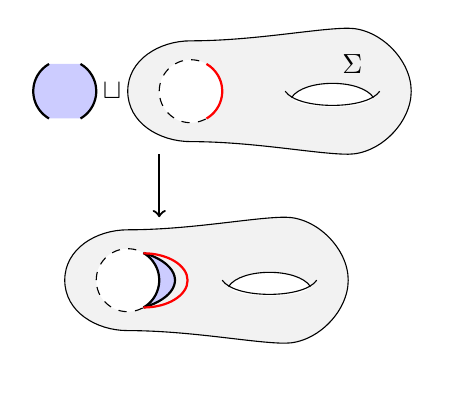
\begin{tikzpicture}[yscale = 0.8, xscale = -0.8]
\fill[gray!10] (4.5,1) .. controls (4.5,0.5) and (4,0.2) .. (3.5,0.2)	.. controls (2.5,0.2) and (1.5,0 ) .. (1,0)	.. controls (0.5,0 ) and (0,0.5 ) .. (0,1)	.. controls (0,1.5 ) and (0.5,2 ) .. (1,2)	.. controls (1.5,2 ) and (2.5,1.8) .. (3.5,1.8) .. controls (4,1.8) and (4.5,1.5) .. (4.5,1) -- cycle ;
\fill[white] (0.6,0.9) .. controls (0.7,0.7) and (1.8,0.7) .. (1.9,0.9) .. controls (1.7,1.2) and (0.8,1.2) .. (0.6,0.9);
\fill[white] (3.5,1) circle(0.5);
\draw[dashed] (3.5,1) circle(0.5);
\draw[thick, red] (240:0.5)++(3.5,1) arc(240:120:0.5);
\draw (0.5,1) .. controls (0.7,0.7) and (1.8,0.7) .. (2,1);
\draw (0.6,0.9) .. controls (0.8,1.2) and (1.7,1.2) .. (1.9,0.9) node[midway, above right]{$\Sigma$};
\draw (4.5,1) .. controls (4.5,0.5) and (4,0.2) .. (3.5,0.2)	.. controls (2.5,0.2) and (1.5,0 ) .. (1,0)	.. controls (0.5,0 ) and (0,0.5 ) .. (0,1)	.. controls (0,1.5 ) and (0.5,2 ) .. (1,2)	.. controls (1.5,2 ) and (2.5,1.8) .. (3.5,1.8) .. controls (4,1.8) and (4.5,1.5) .. (4.5,1);
\node (sq) at (4.75,1){$\sqcup$}; \draw[->, thick] (4,0) -- ++(0,-1) node[midway, right]{};
\fill[blue!20](240:0.5)++(5.5,1) arc(240:120:0.5) -- ++(0.5,0) arc(60:-60:0.5) -- ++(-0.5,0);
\draw[thick] (240:0.5)++(5.5,1) arc(240:120:0.5);
\draw[thick] (-60:0.5)++(5.5,1) arc(-60:60:0.5);
\begin{scope}[yshift = -3cm, xshift = 1cm]
\fill[gray!10] (4.5,1) .. controls (4.5,0.5) and (4,0.2) .. (3.5,0.2)	.. controls (2.5,0.2) and (1.5,0 ) .. (1,0)	.. controls (0.5,0 ) and (0,0.5 ) .. (0,1)	.. controls (0,1.5 ) and (0.5,2 ) .. (1,2)	.. controls (1.5,2 ) and (2.5,1.8) .. (3.5,1.8) .. controls (4,1.8) and (4.5,1.5) .. (4.5,1) -- cycle ;
\fill[white] (0.6,0.9) .. controls (0.7,0.7) and (1.8,0.7) .. (1.9,0.9) .. controls (1.7,1.2) and (0.8,1.2) .. (0.6,0.9);
\fill[white] (3.5,1) circle(0.5);
%\fill[white] (240:0.5)++(3.5,1) arc(240:120:0.5) arc(90:270:0.7 and 0.43);
\fill[blue!20] (240:0.5)++(3.5,1) arc(240:120:0.5) arc(120:240:1 and 0.5);
\draw[dashed] (3.5,1) circle(0.5);
\draw[thick] (240:0.5)++(3.5,1) arc(240:120:0.5);
\draw[thick] (240:0.5)++(3.5,1) arc(240:120:1 and 0.5);
\draw[thick, red] (240:0.5)++(3.5,1) arc(270:90:0.7 and 0.43);
\draw (0.5,1) .. controls (0.7,0.7) and (1.8,0.7) .. (2,1);
\draw (0.6,0.9) .. controls (0.8,1.2) and (1.7,1.2) .. (1.9,0.9) node[midway, above right]{};
\draw (4.5,1) .. controls (4.5,0.5) and (4,0.2) .. (3.5,0.2)	.. controls (2.5,0.2) and (1.5,0 ) .. (1,0)	.. controls (0.5,0 ) and (0,0.5 ) .. (0,1)	.. controls (0,1.5 ) and (0.5,2 ) .. (1,2)	.. controls (1.5,2 ) and (2.5,1.8) .. (3.5,1.8) .. controls (4,1.8) and (4.5,1.5) .. (4.5,1);
\end{scope}
\end{tikzpicture}
$$
To simplify notation, we write ${\rm SK}_\mathcal{V}(-) := \Free({\rm Sk}_\mathcal{V}(-))$ and still denote the action functor on free cocompletions by $\rhd\colon \mathcal{E} \boxtimes {\rm SK}_\mathcal{V}(\Sigma)\to {\rm SK}_\mathcal{V}(\Sigma)$. For $M_1$ and $M_2$ two objects of ${\rm Sk}_\mathcal{V}(\Sigma)$, one has an internal $\Hom$ object $\undHom(M_1,M_2) \in \mathcal{E}$.

\begin{Definition}
Let $\Sigma$ be a surface with boundary with a chosen thickened arc on its boundary.
The internal skein algebra $A_\Sigma := \undHom(\varnothing,\varnothing)$ is the endomorphism algebra of $\varnothing \in {\rm Sk}_\mathcal{V}(\Sigma) \subseteq {\rm SK}_\mathcal{V}(\Sigma)$ with respect to the $\mathcal{E}$-module structure. Its algebra structure is recalled in Definition~\ref{algStrOnIntHom}.
Explicitly, $A_\Sigma$ comes equipped with a natural isomorphism $\sigma \colon \Hom_{{\rm SK}_\mathcal{V}(\Sigma)}(-\rhd \varnothing, \varnothing) \tilde{\Rightarrow} \Hom_{\mathcal{E}}(-, A_\Sigma)$ between (contravariant) functors $\mathcal{E}\to {\rm Vect}_k$.
If $\mathcal{V} = \Oq\text{-}{\rm comod}^{\rm fin}$ with $\mathcal{E}=\Oq\text{-}{\rm comod}$, then $A_\Sigma$ is an $\Oq$-comodule algebra.
\end{Definition}

\begin{Remark}\label{rmkTopPtsAndASigma}
The defining properties of $A_\Sigma$ enables one to describe morphisms $V \rhd \varnothing \to \varnothing$ in ${\rm Sk}_\mathcal{V}(\Sigma)$, so where the boundary points of tangles are at the bottom, as morphisms $V \to \mathscr{S}(\Sigma)$ in $\mathcal{E}$. We would also like to describe morphisms $W\rhd \varnothing \to V \rhd \varnothing$ in ${\rm Sk}_\mathcal{V}(\Sigma)$. By duality in~$\mathcal{V}$, the functor $V\rhd-$ is right adjoint to $V^*\rhd-$, see \cite[Proposition~7.1.6]{EGNO}. So one has natural isomorphisms:
\begin{align*}
\Hom_{{\rm Sk}_\mathcal{V}(\Sigma)}(W\rhd\varnothing, V \rhd\varnothing) &\,\tilde{\to} \, \Hom_{{\rm Sk}_\mathcal{V}(\Sigma)}(V^*\rhd( W \rhd \varnothing), \varnothing) \overset{\sigma_{V^*\otimes W}}{\to} \Hom_{\mathcal{E}}(V^*\otimes W, A_\Sigma)
\\
&\, \tilde{\to} \, \Hom_{\mathcal{E}}(W,V\otimes A_\Sigma).
\end{align*}
When $\Sigma$ is connected, every object of ${\rm Sk}_\mathcal{V}(\Sigma)$ is isomorphic to one of the form $V\rhd\varnothing$, and the above natural isomorphism suggests that the algebra $A_\Sigma\in\mathcal{E}$ is enough to fully describe ${\rm SK}_\mathcal{V}(\Sigma)$.
\end{Remark}
